\chapter{Capacitance}

A capacitor ``is a device that stores energy in an electrostatic field.'' Capacitors, in general, are made of two metal sheets separated by a dielectric and wrapped in a cylinder. In fact, any two conductive elements not in contact can form a capacitor. When we create a potential difference across these two elements, charges will move from high potential to low potential. With this behavior, capacitors can be seen as a conductor in a circuit that can also be used to store energy. At any instance in time, there are equal amount of charges (positive or the two plates (conductive elements) of the capacitor, given a neutral capacitor and a circuit context. The accumulation of charge is charging the capacitor; vice versa, the charge/energy stored can also be discharged.

Real world capacitors have internal resistance, theoretically modelled capacitors, however, are ideal and do not have resistance. Thus, we consider RC (Resistor, Capacitor) circuits instead of circuits with only the emf and capacitor (this will theoretically cause the capacitor to charge up instantly with infinite current).

Capacitance is first modelled by the relation

\[Q = CV\]

where C is the capacitance measured in \textbf{farads}, Q is the amount of charge to fully charge the capacitor, and V is the voltage given across the capacitor.

Consider the following circuit

\begin{center}
    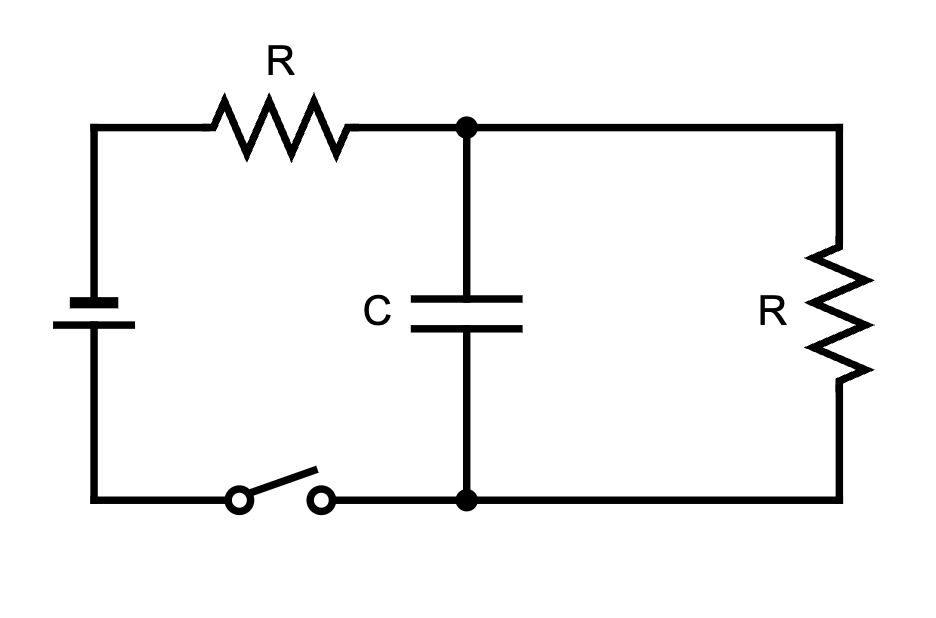
\includegraphics[scale=0.35]{assets/rc-circuit}
\end{center}

We have a switch to break the emf from the circuit, capacitor, and two resistors. 

\section{Charging the Capacitor}

Applying Kirchhoff's Law on the left loop with the switch closed, we obtain 

\begin{align*}
    \mathcal{E} - V_C - IR &= 0\\
    \mathcal{E} - \frac{Q}{C} &= \frac{\dif Q}{\dif t} R\\
    \int \frac{\dif t}{R} &= \int \frac{\dif Q}{\mathcal{E} - \frac{Q}{C}}\\
    \frac{t}{R} + C_1 &= -C \ln\abs{\mathcal{E} - \frac{Q}{C}}\\
    -\frac{t}{RC} + C_1 &= \ln\abs{\mathcal{E} - \frac{Q}{C}}\\
    Ae^{-\frac{t}{RC}} &= \mathcal{E} - \frac{Q}{C}\\
    Q(t) &= C \left(\mathcal{E} - Ae^{-\frac{t}{RC}}\right)
\end{align*}

we apply the fact that the capacitor is uncharged at $t = 0$

\[\boxed{Q(t) = C \mathcal{E} \left(1 - e^{-\frac{t}{RC}}\right)}\]

Taking the derivative yields the function of current over time, which is also exponential

\begin{align*}
    Q'(t) = I(t) &= \frac{\dif}{\dif t} C \mathcal{E} \left(1 - e^{-\frac{t}{RC}}\right)\\
    &= \boxed{\frac{\mathcal{E}}{R} e^{-\frac{t}{RC}}}
\end{align*}

Here's a graph from \href{http://hyperphysics.phy-astr.gsu.edu/hbase/hph.html}{Hyper Physics}

\begin{center}
    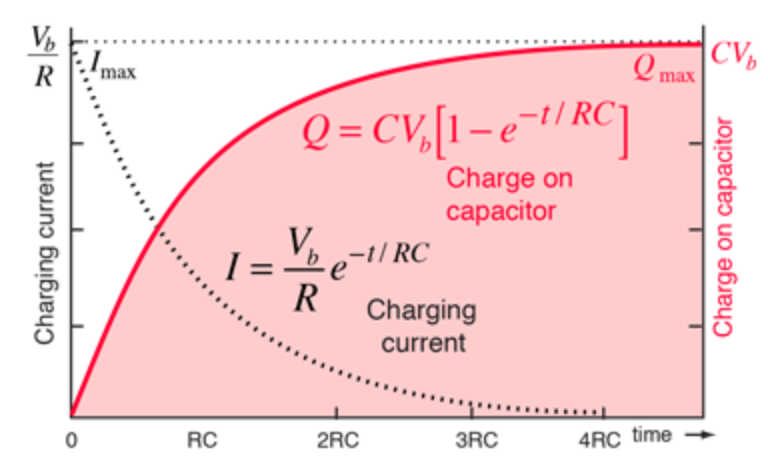
\includegraphics[scale=0.6]{assets/hp-c-charging.png}
\end{center}

\section{Discharging the Capacitor}

Applying Kirchhoff's Law on the right loop (and with some substitution), we obtain 

\begin{align*}
    V_C - IR &= 0\\
    \frac{Q}{C} &= \frac{-\dif Q}{\dif t} R\\
    -\frac{\dif t}{RC} &= \frac{\dif Q}{Q}\\
    -\frac{t}{RC} + C_1 &= \ln\abs{Q}\\
    Q(t) &= C_1 e^{-\frac{t}{RC}}\\
    &= Q_0 e^{-\frac{t}{RC}}\\
    &= \boxed{CV_0 e^{-\frac{t}{RC}}}
\end{align*}

Not that $I$ is $-\dif Q / \dif t$ but not $\dif Q / \dif t$ because, as the capacitor is discharging, the current is positive on the resistor; change of charge on the capacitor $\dif Q_c$, however, is negative. We need to, thus, govern that relationship.

Here's a graph from \href{http://hyperphysics.phy-astr.gsu.edu/hbase/hph.html}{Hyper Physics}

\begin{center}
    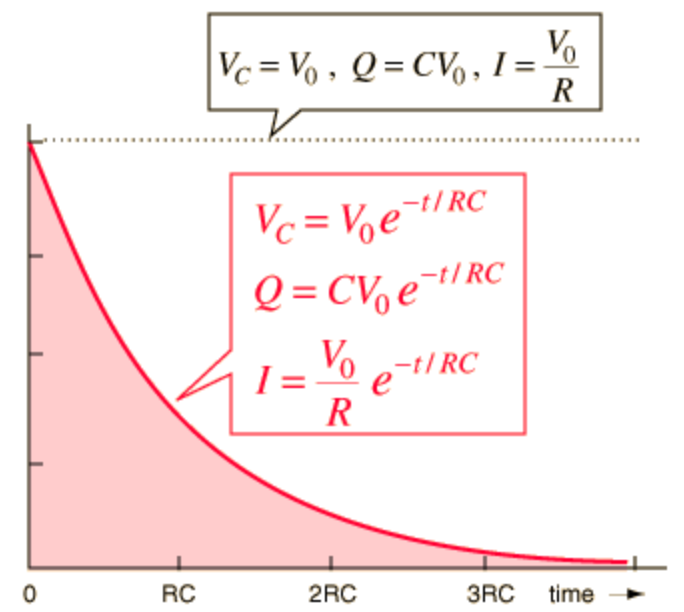
\includegraphics[scale=0.6]{assets/hp-c-discharging.png}
\end{center}

\section{RC Time Constant}

In the exponential functions derived above, we see the the common existence of the $RC$ expression; this is called the \textbf{RC Time Constant}. In general, there is a $63.2\%$ change at $t = RC$, a $86.5\%$ change at $t = 2RC$, and a $95.0\%$ change at $t = 3RC$.

Considering the numerical value of the time constant: the greater $RC$ is, the longer it takes for the capacitor to charge up or discharge.

\section{Energy}

There are many ways to find energy stored by a capacitor, there are, for example, two ways that I know of:
\begin{enumerate}[1.]
    \item By utilizing the relation $P = IV = I^2R$ to sum the power over time, which is energy, of some resistor in an RC circuit.
    \item By summing up the energy of moving all the charges for a capacitor.
\end{enumerate}

For the first method:

\begin{align*}
    U = W &= \int P \,\dif t\\
    &= \int I^2R \,\dif t\\
    &= \int_0^\infty \left(\frac{V_0}{R} e^{-\frac{t}{RC}}\right)^2 R \,\dif t\\
    &= \left.-\frac{1}{2} C{V_0}^2 e^{-\frac{2t}{RC}}\right\vert_0^\infty\\
    &= \boxed{\frac{1}{2} C{V_0}^2 = \frac{1}{2} \frac{Q^2}{C} = \frac{1}{2}QV_0}\\
\end{align*}

For the second method we can see this as moving charge across a certain potential (given by the amount of charge on the plates). The work done will then be

\[\dif W = V(q) \dif q\]

The total work to move all the charges:

\begin{align*}
    U  = W &= \int_0^Q V(q) \,\dif q\\
    &= \int_0^Q \frac{q}{C} \,\dif q\\
    &= \boxed{\frac{1}{2} \frac{Q^2}{C} = \frac{1}{2}CV^2 = \frac{1}{2}QV}
\end{align*}

\section{Finding Capacitance}

We know a relation of capacitance

\[Q = CV\]



\section{Dielectric and the Dielectric Constant}

When we add some dielectric between the plates of the capacitor, the electron of the atoms of the dielectric will be at an offset caused by the electrical field of the plates. In other words, they are \textit{polarizable}. This creates an opposing electric field to those created by the plates. Thus, to maintain the same voltage across the plates (to the emf), the charge density of the plates have to increase, causing more charge to be on the capacitor. This directly affects the capacitance and is measured by the \textbf{dielectric constant}, also called \textbf{relative permittivity}: $\kappa$

\[\kappa = \frac{\varepsilon}{\varepsilon_0}\]

where $\varepsilon$ is the permittivity of the material/dielectric, and $\varepsilon_0$ is the permittivity of vacuum.

Capacitance can be found with

\[C = \kappa C_0\]

where $C$ is the capacitance of the capacitor with dielectric, and $C_0$ is the capacitance of capacitor with vacuum.

\section{Capacitor Circuits}

\subsection{Series}

\hfil 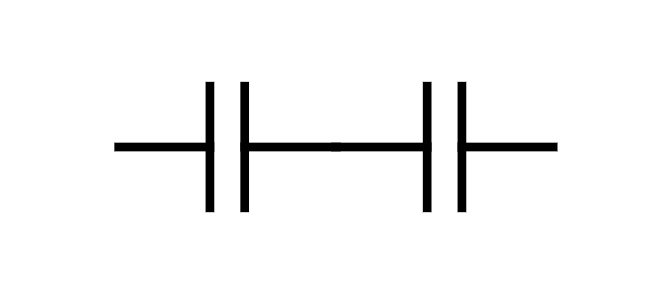
\includegraphics[scale=0.35]{assets/c-series.png}

\subsection{Parallel}

\hfil 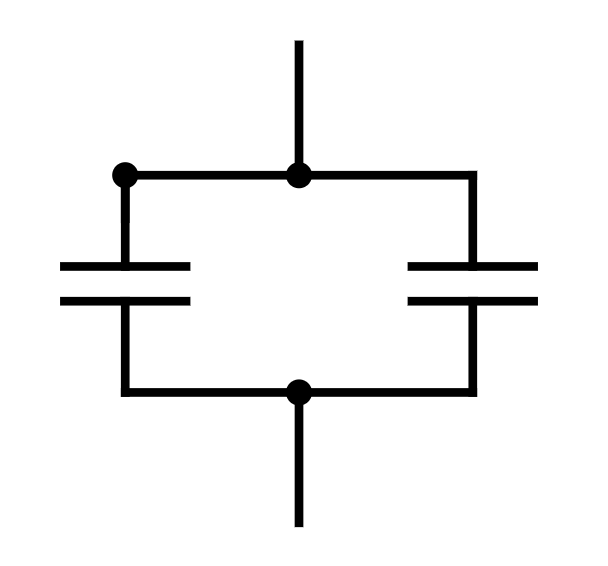
\includegraphics[scale=0.35]{assets/c-parallel.png}